\documentclass[crop,tikz,10pt]{standalone}

\usepackage{tikz-qtree}

\usetikzlibrary{calc}
\usetikzlibrary{positioning}
\usetikzlibrary{arrows.meta}
\usetikzlibrary{decorations.text}
\usetikzlibrary{backgrounds}

\definecolor{bg1}{RGB}{244,231,195}
\definecolor{bg2}{RGB}{234,204,161}
\definecolor{l1}{RGB}{209,148,106}

\begin{document}

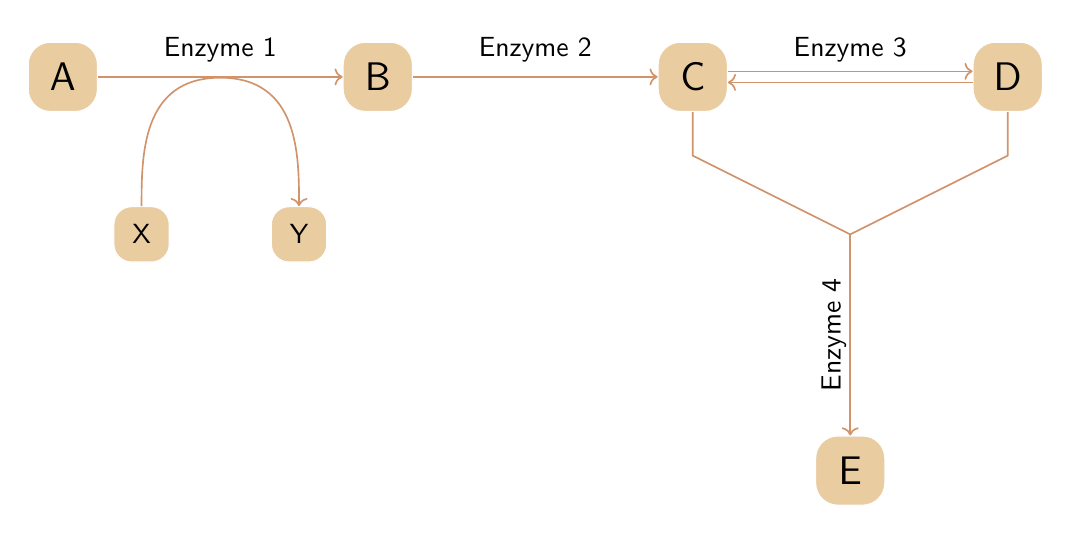
\begin{tikzpicture}[
    font=\sffamily,
    a/.style={
        line width=0.6pt,
        color=l1,
    },
    l/.style={
        a,-{Computer Modern Rightarrow[line width=0.6pt]}
    },
    m/.style={
        fill=bg2, draw=white, line width=0.4pt,
        rounded corners=8pt, minimum size=2.5em,
        font=\sffamily\Large
    },
    s/.style={
        m, rounded corners=6.4pt, minimum size=2em,
        font=\sffamily\normalsize
    },
    e/.style={
        midway,yshift=10pt,color=black
    }
]

    \node [m] (a) at ( 0  ,  0) {A};
    \node [m] (b) at ( 4  ,  0) {B};
    \node [m] (c) at ( 8  ,  0) {C};
    \node [m] (d) at (12  ,  0) {D};
    \node [m] (e) at (10  , -5) {E};
    \node [s] (x) at ( 1, -2) {X};
    \node [s] (y) at ( 3, -2) {Y};
    
    \draw (a) -- (b) [l] node [e] {Enzyme 1};
    \draw (b) -- (c) [l] node [e] {Enzyme 2};
    \draw (c) -- (d) [l,transform canvas={yshift=2pt}] node [e,yshift=-2pt] {Enzyme 3};
    \draw (d) -- (c) [l,transform canvas={yshift=-2pt}];
    \draw (c) -- ++ (0, -1)  -- (10, -2) [a];
    \draw (d) -- ++ (0, -1)  -- (10, -2) [a];
    \draw (10, -2) -- (e) [l] node [midway,color=black,rotate=90,yshift=6pt] {Enzyme 4};
    
    \draw (x) .. controls (1,-1) and (1,-0.3pt) .. (2, -0.3pt) [a];
    \draw (2, -0.3pt) .. controls (3,-0.3pt) and (3,-1) .. (y) [l];
    
    % \draw (e.west) .. controls (7, -5) and (6, -4) .. (6, -1) -- (6, -0.2) [a,-{|[width=10]}];
    
    % \node [e] (A) at ( 0.5,  0) {A};
    % \node [e] (B) at (-2  , -1) {B};
    % \node [e] (C) at ( 3  , -1) {C};
    % \node [e] (D) at (-3.5, -2) {D};
    % \node [e] (E) at (-2  , -2) {E};
    % \node [e] (F) at (-0.5, -2) {F};
    % \node [e] (G) at ( 1.5, -2) {G};
    % \node [e] (H) at ( 4  , -2) {H};
    % \node [e] (I) at (-4  , -3) {I};
    % \node [e] (J) at (-2  , -3) {J};
    % \node [e] (K) at ( 0  , -3) {K};
    % \node [e] (L) at ( 1  , -3) {L};
    % \node [e] (M) at ( 2  , -3) {M};
    % \node [e] (N) at ( 4  , -3) {N};
    % \node [e] (O) at (-4.5, -4) {O};
    % \node [e] (P) at (-3.5, -4) {P};
    % \node [e] (Q) at (-2  , -4) {Q};
    % \node [e] (R) at ( 0.5, -4) {R};
    % \node [e] (S) at ( 2.5, -4) {S};
    % \node [e] (T) at ( 4  , -4) {T};
    
    % \draw (A) edge [l] (B);
    % \draw (A) edge [l] (C);
    % \draw (B) edge [l] (D);
    % \draw (B) edge [l] (E);
    % \draw (B) edge [l] (F);
    % \draw (C) edge [l] (G);
    % \draw (C) edge [l] (H);
    % \draw (D) edge [l] (I);
    % \draw (D) edge [l] (J);
    % \draw (E) edge [l] (J);
    % \draw (F) edge [l] (K);
    % \draw (G) edge [l] (L);
    % \draw (G) edge [l] (M);
    % \draw (H) edge [l] (N);
    % \draw (I) edge [l] (O);
    % \draw (I) edge [l] (P);
    % \draw (J) edge [l] (Q);
    % \draw (K) edge [l] (R);
    % \draw (L) edge [l] (R);
    % \draw (M) edge [l] (S);
    % \draw (N) edge [l] (T);
    
\end{tikzpicture}

\end{document}
